\documentclass[12pt]{article}
%\usepackage{geometry}                % See geometry.pdf to learn the layout options. There are lots.
%\geometry{letterpaper}                   % ... or a4paper or a5paper or ... 
%\geometry{landscape}                % Activate for for rotated page geometry
\usepackage[parfill]{parskip}    % Activate to begin paragraphs with an empty line rather than an indent
\usepackage{daves,fancyhdr,natbib,graphicx,dcolumn,amsmath,lastpage,url}
\usepackage{amsmath,amssymb,epstopdf,longtable}
\usepackage{paralist}  % need to properly formulate standard answer blocks
\usepackage[final]{pdfpages}
\usepackage{multicol}
\usepackage{booktabs}
\DeclareGraphicsRule{.tif}{png}{.png}{`convert #1 `dirname #1`/`basename #1 .tif`.png}
\pagestyle{fancy}
\lhead{CE 3372 Water Systems Design}
\rhead{}
\lfoot{REVISION A}
\cfoot{}
\rfoot{Page \thepage\ of \pageref{LastPage}}
\renewcommand\headrulewidth{0pt}

%%%%%%%%%% Will's listing environment %%%%%%%
\usepackage[left=1.25in, right=1.25in,
            top=1in, bottom=1in]{geometry}                % See geometry.pdf to learn the layout options. There are lots.
\geometry{letterpaper}

\usepackage{ragged2e}

\usepackage{xcolor}
\newcommand{\codeRcolor}{0.93}
\newcommand{\codeGcolor}{0.93}
\newcommand{\codeBcolor}{0.93}
\definecolor{lightgrey}{rgb}{\codeRcolor,
                             \codeGcolor,
                             \codeBcolor}

\newcommand{\listingfont}{\fontsize{7pt}{8pt}\selectfont\ttfamily}
\usepackage{listings}
\lstset{basicstyle = \listingfont,
        breaklines = true,
        frame=tb,
        xleftmargin=12pt,
        framexleftmargin=6pt,
        framexrightmargin=6pt,
        xrightmargin=12pt,
        columns=fixed}
\lstset{lineskip=-1pt}
\lstset{backgroundcolor=\color{lightgrey}}


\usepackage[font={footnotesize},
            labelfont={sf,bf},
            textfont={sf},
            singlelinecheck=false,
            labelsep=none,
            justification=RaggedRight,
            aboveskip=0pt,
            belowskip=7pt plus 1pt minus 1pt,
            textformat=period]{caption}
\DeclareCaptionLabelSeparator{mystyle}{.\quad}
\captionsetup{labelsep=mystyle}
%%%%%%%%% End Will's listing environment ABOVE %%%%%%%%%

\begin{document}
%%%%%%%%%%%%%%%%%%%%%%%%%%%%%%%%%%%
\begingroup
\begin{center}
{\textbf{{ CE 3372 Water Systems Design} \\  Drainage Design by Rational Method for Sizing Storm Sewer Pipes }}
\end{center}
\endgroup
\section*{Introduction}
The size selection of storm sewer pipes for small systems is usually accomplished using the Rational Runoff Equation in conjunction with Manning's Equation to construct an initial design for a drainage network.  
The initial design that results should be checked with a hydraulic analysis to be sure the design will actually accomplish the hydraulic objectives, and to account for outfall conditions, backwater effects, and similar hydraulic situations that are beyond the initial estimated from the Rational Equation.
Usually the preliminary design does indeed perform as-is in the hydraulic model, but not always.

Here we illustrate the method by an example.  
The method employed here is described in some detail in \cite{Wurbs2002},\cite{Chin2006}, and \cite{mays2011}.

\section*{Problem Statement}
\label{prob:drainDesign} Consider the three drainage areas that drain to the inlets connected to the pipes as shown in Figure \ref{fig:DrainageLayout}.  
A stormwater drainage system is being designed to carry the flow from the three areas.  
\begin{figure}[ht!] %  figure placement: here, top, bottom, or page
\centering
   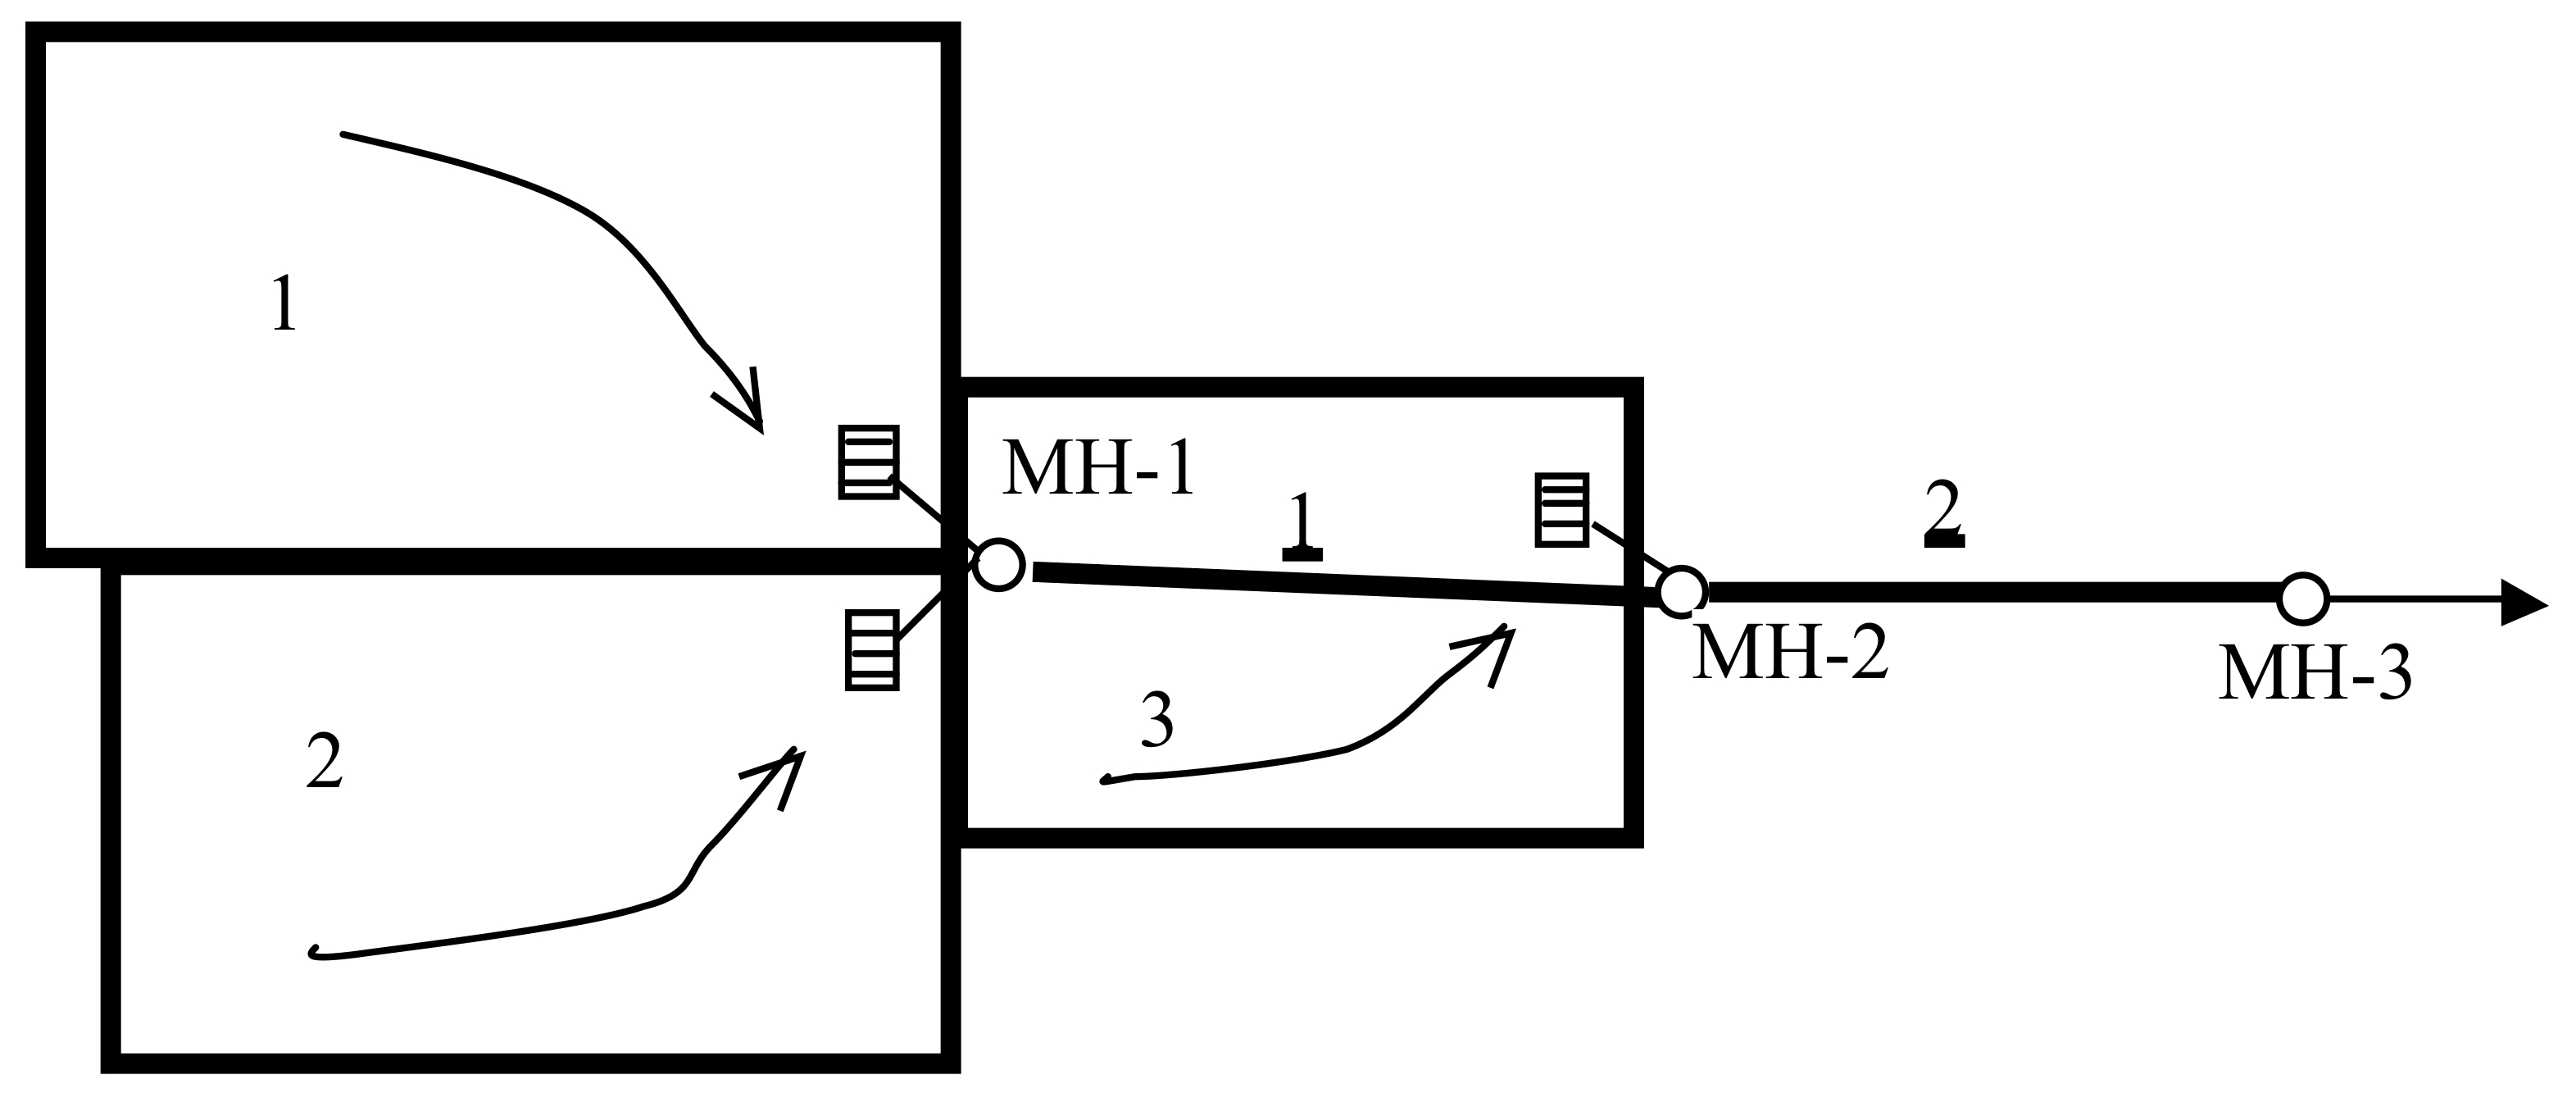
\includegraphics[width=6in]{DrainageLayout.jpg}
   \caption{Drainage System Layout}
   \label{fig:DrainageLayout} 
\end{figure}
Table \ref{tab:drainageArea} lists drainage area information.\\
% Requires the booktabs if the memoir class is not being used
\begin{table}[h!]
   \centering
   \caption{Contributing Area Information}
   \begin{tabular}{c c c c} % Column formatting, @{} suppresses leading/trailing space
   ~ & ~ & ~ & \\
   \hline
   \hline
      Area ID & Area (acres) & C (runoff coefficient) & Inlet Time (minutes) \\
      \hline
      DA-1 & 6.0 & 0.65 & 17 \\
      DA-2 & 5.1 & 0.55 & 14 \\
      DA-3 & 3.5 & 0.70 & 12 \\
      \hline
      \hline
   \end{tabular}
   \label{tab:drainageArea}
\end{table}

Table \ref{tab:pipes} lists pipe information.\\

\begin{table}[h!]
   \centering
   \caption{Pipe Information}
   \begin{tabular}{c c c c c c} % Column formatting, @{} suppresses leading/trailing space
   ~ & ~ & ~ & ~ & ~ & \\
   \hline
   \hline
      Pipe\_ID & Upstream Junction & Downstream Junction & Length (feet) & Slope & Manning's $n$ \\
      \hline
     P1 &  MH-1 & MH-2 & 600 & 0.003 & 0.015 \\
     P2 &  MH-2 & MH-3 & 600 & 0.003 & 0.015 \\
      \hline
      \hline
   \end{tabular}
   \label{tab:pipes}
\end{table}

The allowable velocity at design flow is between 2 and 10 feet-per-second.

The 10-year ARI intensity equation for the area is given in Equation \ref{eqn:intensity}, where $I$ is intensity in inches-per-hour, and $T_c$ is the averaging time, in minutes.

\begin{equation}
I = \frac{56.6}{(T_c + 8.6)^{0.823}}
\label{eqn:intensity}
\end{equation}
 
Determine the design flow rates in cfs and diameters in inches for both pipes using the Rational Method Storm Sewer Design procedure described in \cite{mays2011}.

\section*{Solution}
The solution presented here is a by-hand approach.
\subsection*{Build Auxiliary Equations}
The method will employ the rational runoff equation, but will also use Manning's equation in several forms.  
Manning's equation will be used to find pipe diameters given discharge, and flow velocities in those pipes based on those diameters, so it is useful to construct these equations before beginning the actual design process.

Equation \ref{eqn:manningsQ} is Manning's equation for a \textbf{full} circular pipe.
\begin{equation}
Q = \frac{1.49}{n} (\frac{\pi D^2}{4})(\frac{D}{4}^{2/3}) S_o^{1/2}
\label{eqn:manningsQ}
\end{equation}

If we rearrange the equation for diameter we obtain Equation \ref{eqn:manningsD}.
\begin{equation}
D = \big[\frac{4^{5/3}~Q~n}{1.49~\pi~S_o^{1/2}}]^{3/8}
\label{eqn:manningsD}
\end{equation}

Equation \ref{eqn:manningsV} is Manning's equation for velocity for a \textbf{full} circular pipe.
\begin{equation}
V = \frac{1.49}{n}(\frac{D}{4})^{2/3} S_o^{1/2}
\label{eqn:manningsV}
\end{equation}

In the problem statement the two pipe slopes are the same as are their Manning's $n$ values, so we can insert them into the equations directly and obtain for \textbf{this example} and obtain

\begin{equation}
D = (0.3958~Q)^{3/8}
\label{eqn:manningsD}
\end{equation}

\begin{equation}
V = 5.44~(\frac{D}{4})^{2/3}
\label{eqn:manningsV}
\end{equation}
\clearpage
\subsection*{Draw the Collection System}
The next step is to draw the collection system topology.
My rules for drawing are:
\begin{enumerate}
\item Draw each drainage area and label it with its area in acres and its runoff coefficient.
Use a mark to indicate the inlet that it drains to.
Label the local $t_c$ as ``inlet time'', $t_{inlet}$.
Figure \ref{fig:DrainageLayout1} illustrates this step for the example.
\begin{figure}[ht!] %  figure placement: here, top, bottom, or page
\centering
   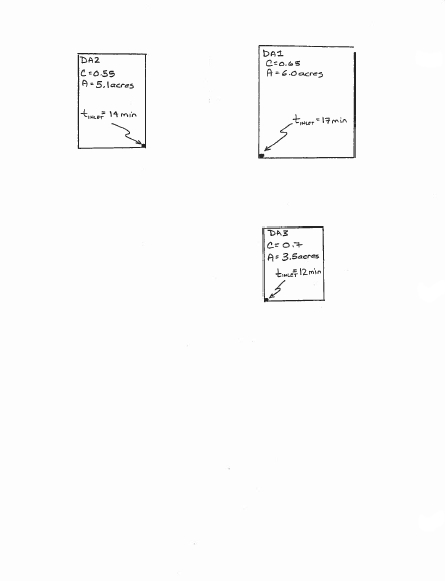
\includegraphics[height=7in]{DrainageLayout1.jpg}
   \caption{By-Hand Drainage System Worksheet.  Drawing the Drainage Areas.}
   \label{fig:DrainageLayout1} 
\end{figure}
\clearpage
\item Draw each junction (node) as a small circle.
label each junction.
Leave space between the node and other objects.
Figure \ref{fig:DrainageLayout2} illustrates this step for the example.
\begin{figure}[ht!] %  figure placement: here, top, bottom, or page
\centering
   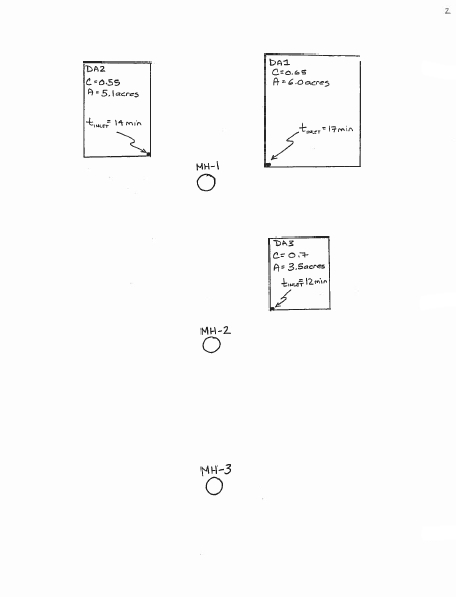
\includegraphics[height=7in]{DrainageLayout2.jpg}
   \caption{By-Hand Drainage System Worksheet. Adding the Junctions.}
   \label{fig:DrainageLayout2} 
\end{figure}
\clearpage
\item Draw each pipe as a small line segment.
Label the segment with a pipe name, and indicate distance if known.
Leave space between the pipes and other objects.
Figure \ref{fig:DrainageLayout3} illustrates this step for the example.
\begin{figure}[ht!] %  figure placement: here, top, bottom, or page
\centering
   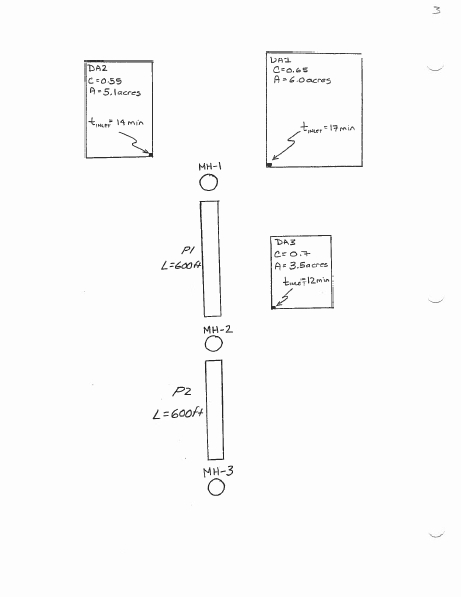
\includegraphics[height=7in]{DrainageLayout3.jpg}
   \caption{By-Hand Drainage System Worksheet. Adding the Pipes.}
   \label{fig:DrainageLayout3} 
\end{figure}
\clearpage
\item Use dashed lines to indicate a connection from a drainage area (inlet) to a junction.
These lines indicate connectivity, but have zero ``length'' in a travel time sense.
Figure \ref{fig:DrainageLayout4} illustrates this step for the example.
\begin{figure}[ht!] %  figure placement: here, top, bottom, or page
\centering
   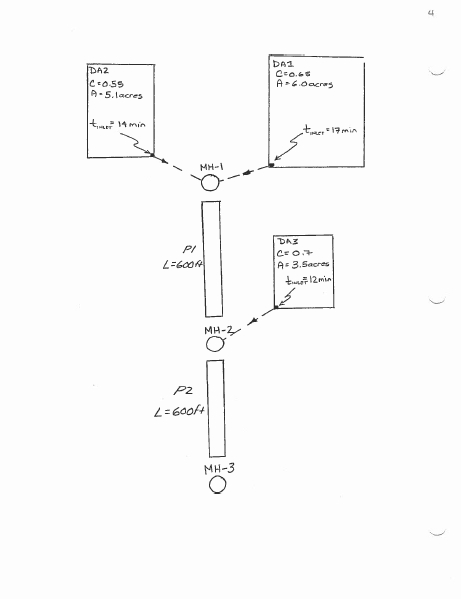
\includegraphics[height=6in]{DrainageLayout4.jpg}
   \caption{By-Hand Drainage System Worksheet. Connecting the Drainage Areas.}
   \label{fig:DrainageLayout4} 
\end{figure}
\end{enumerate}

\subsection*{Compute $CA$ values}
The next step is to determine the $CA$ values for each drainage area and the accumulating $\sum (CA)_i$ as one traverses downstream in the drainage network.

A suggested procedure is to: ~\newpage
\begin{enumerate}
\item Compute the product of $C$ and $A$ for each drainage area.
List the value at the drainage area outlet (which will be a sewer inlet).
Figure \ref{fig:DrainageLayout5} illustrates this step for the example.
\begin{figure}[ht!] %  figure placement: here, top, bottom, or page
\centering
   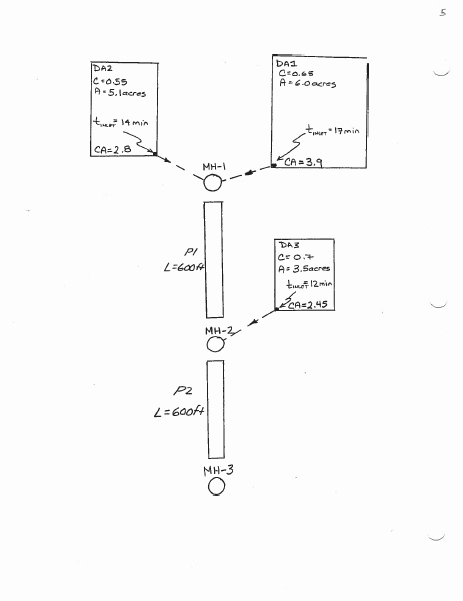
\includegraphics[height=7in]{DrainageLayout5.jpg}
   \caption{By-Hand Drainage System Worksheet. Computing the $CA$ values.}
   \label{fig:DrainageLayout5} 
\end{figure}
\clearpage
\item When all the drainage areas are labeled, starting at the most upstream drainage area, find the junction the drainage area connects to and accumulate the sum of all $CA$ values to that junction, including any area that is connected by an upstream pipe.   
List the $\sum (CA)_i$ next to the junction so you can refer to the value later on in the procedure.
Figure \ref{fig:DrainageLayout6} illustrates this step for the example.
\begin{figure}[ht!] %  figure placement: here, top, bottom, or page
\centering
   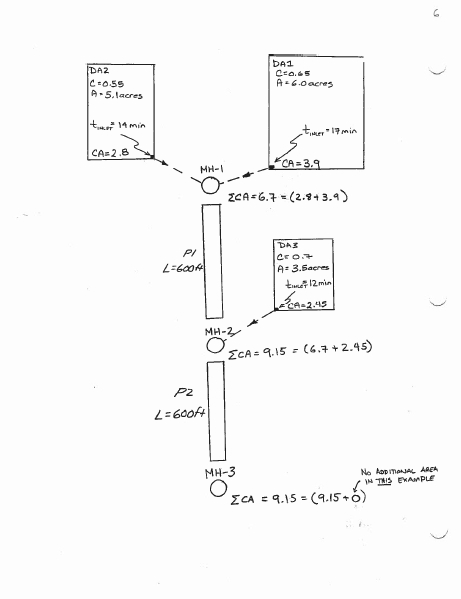
\includegraphics[height=7in]{DrainageLayout6.jpg}
   \caption{By-Hand Drainage System Worksheet. Computing the $\sum (CA)_i$ values.}
   \label{fig:DrainageLayout6} 
\end{figure}
\end{enumerate}

\subsection*{Compute $Q_{junction}$, $D_{pipe}$,$V_{pipe}$, and $t_{pipe}$}
The next step is to compute the discharge leaving each junction and the various pipe parameters of the pipe connected \textbf{downstream} of the junction.
Observe how the topology was drawn; flow leaves a junction and enters a sewer conduit, so the flow leaving a junction will be the flow that enters the pipe downstream of that junction. 
We will use that flow value to determine the pipe travel time as we proceed downstream.
\begin{enumerate}
\item Starting at the most upstream junction, determine the $t_c$ to use for the rational method as the longer of local inlet times (time associated with any directly connected drainage area) or the total accumulated travel time to the junction.
\begin{equation}
t_c = max( t_{i,local},t_{up})
\end{equation}
\item Apply that $t_c$ in the rational equation and use the $\sum (CA)_i$ value at the junction to determine the discharge leaving the junction.
\item Write that discharge as the discharge in pipe immediately downstream of the junction.
\item Use that discharge to compute the full pipe diameter.  Write the value next to the pipe.
\item Use the diameter to compute the full pipe velocity. Write the value next to the pipe.
\item Compute the pipe travel time $t_{pipe} = \frac{L_{pipe}}{V_{pipe}}$; express the result in minutes.
\item Move to the next junction.  If you reach a junction which has un-calculated upstream contribution, complete the upstream contribution calculations before proceeding to the next junction.
\item Repeat steps 1 through 6 to find the pipe time (and flows) to the next junction. 
\end{enumerate}

The designer repeats the steps above, iteratively as needed until the entire network has been traversed from upstream to the outfall.  
The resulting values constitute an initial guess for a design.

The next several pages show these steps for the example problem.

\newpage
Figure \ref{fig:DrainageLayout7} illustrates Step 1 for $MH-1$, the longest time in this instance is the inlet time for $DA-1$.  Because $DA-1$ and $DA-2$ both connect to the junction, we will use the $\sum (CA)_i$ value we have already computed for the junction.
\begin{figure}[ht!] %  figure placement: here, top, bottom, or page
\centering
   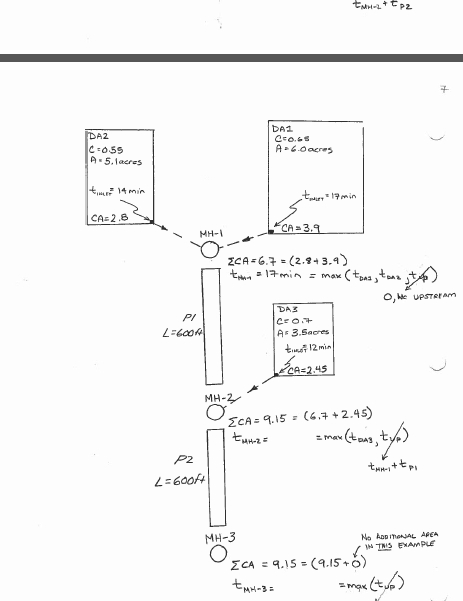
\includegraphics[height=7in]{DrainageLayout7.jpg}
   \caption{By-Hand Drainage System Worksheet. Computing $t_{MH-1}$}
   \label{fig:DrainageLayout7} 
\end{figure}
\clearpage
Figure \ref{fig:DrainageLayout8} illustrates Steps 2-6 for $MH-1$ and $P-1$. 
The computed pipe travel time is 2.57 minutes, and this time is added to $t_{MH-1}$ to become the $t_{UP}$ for the next node time of concentration determination. 

\begin{figure}[ht!] %  figure placement: here, top, bottom, or page
\centering
   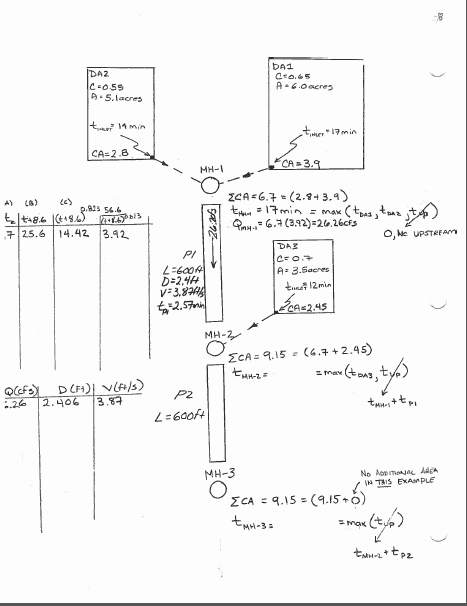
\includegraphics[height=7in]{DrainageLayout8.jpg}
   \caption{By-Hand Drainage System Worksheet. Computing $Q_{MH-1}$, $D_{P1}$, $V_{P1}$, and $t_{P1}$}
   \label{fig:DrainageLayout8} 
\end{figure}
\clearpage
Figure \ref{fig:DrainageLayout9} illustrates Steps 1-6 for $MH-2$ and $P-2$. 
The longest time to $MH-2$ is the larger of the local time from $DA-3$ or the upstream travel time $t_{UP}$.
In this case the longer time is the upstream time, which has a value of 19.57 minutes.
This time is then used in the rational equation, with the $\sum (CA)_i$ for $MH-2$.

\begin{figure}[ht!] %  figure placement: here, top, bottom, or page
\centering
   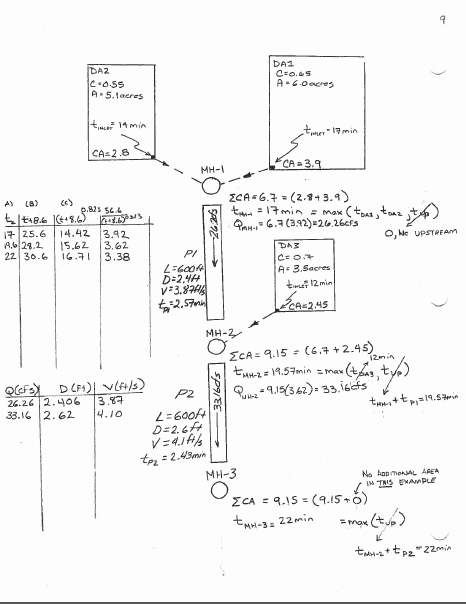
\includegraphics[height=6.5in]{DrainageLayout9.jpg}
   \caption{By-Hand Drainage System Worksheet. Computing $t_{MH-2}$, $Q_{MH-2}$, $D_{P2}$, $V_{P2}$, and $t_{P2}$}
   \label{fig:DrainageLayout9} 
\end{figure}

Once the discharge is computed, the pipe properties are found using Manning's equation to find the pipe diameter and travel time.
The computed pipe travel time is 2.43 minutes which is added to the $t_{MH-2}$ to become the next $t_{UP}$ if we needed to continue the computations further downstream.
\clearpage 
Figure \ref{fig:DrainageLayout10} illustrates the initial design of the system including specification of commercial pipe sizes.

\begin{figure}[ht!] %  figure placement: here, top, bottom, or page
\centering
   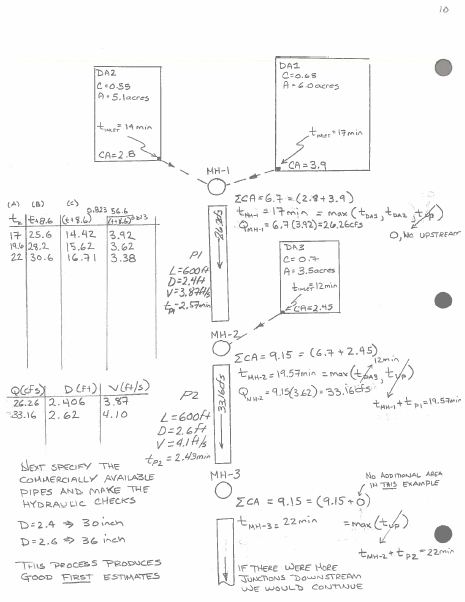
\includegraphics[height=7in]{DrainageLayout10.jpg}
   \caption{By-Hand Drainage System Worksheet. Specification of commercial pipe dimensions.  This represents the initial design.  If behavior at $MH-3$ and beyond were important, then continue the process.}
   \label{fig:DrainageLayout10} 
\end{figure}

Table \ref{tab:designpipes} summarizes the results of the process applied to the example problem. 

This initial design would be subjected to further refinements and checks.
The next step would be to check the hydraulics (and hydrology) using the commercial pipes -- this check will impact the pipe times a little bit, but otherwise the process is unchanged.\footnote{The partial-full pipe equations are used in this check with the known diameters and discharges to compute the average velocities and pipe times.  Then as one moves downstream the $t_c$ change a little bit.  Mostly one should discover that the times don't change very much, neither do the discharges.}

The next step would be to specify invert elevations for the junctions so that the pipes will be underground and buried deep enough to carry any overburden loads that are anticipated.  
These invert elevations are dictated by the outfall elevation, so the step is not trivial.  

Once these elevations are specified, then one will move to a hydraulic model to check effects of downstream boundary conditions, verify that the system will not surcharge, and make adjustments to diameters and elevations to accommodate a design storm.\footnote{This check is what SWMM or HEC-RAS is used for (SWMM is usually the better choice for sewer systems).}


\begin{table}[h!]
   \centering
   \caption{Drainage Preliminary Design}
   \begin{tabular}{p{0.5in}p{0.5in}p{0.4in}p{0.4in}p{0.4in}p{0.4in}p{0.5in}p{0.5in}p{0.4in}p{0.4in}p{0.4in}} % Column formatting, @{} suppresses leading/trailing space
   ~ & ~ & ~ & ~ & ~ & \\
   \hline
   \hline
      Pipe\_ID & Length & Area & $\sum CA$ & $T_C$ & $I$ & Q  & D$_{calc.}$ &  D$_{used}$ & V$_{pipe}$  & 
  T$_{pipe}$ \\
        ~ &  (ft) &  (ac.) & ~&  (min) &  (in/hr) &  (cfs) & (ft) &  (in) &  (ft/s) & 
   (min) \\
      \hline
               ~ &  ~ &  ~ & ~&  ~ &  ~ &  ~& ~ &  ~ &  ~ & ~ \\
         P-1 &  600 &  11.1 & 6.7 & 17 &  3.92 &  26.26 & 2.4 & 30 & 3.87 & 2.57 \\
         ~ &  ~ &  ~ & ~&  ~ &  ~ &  ~& ~ &  ~ &  ~ & ~ \\
         \hline
                           ~ &  ~ &  ~ & ~&  ~ &  ~ &  ~& ~ &  ~ &  ~ & ~ \\
         P-2 &  600 &  14.6 & 9.15 &  19.57 & 3.62 & 33.16 & 2.6 & 36 & 4.1 & 2.43 \\ 
                  ~ &  ~ &  ~ & ~&  ~ &  ~ &  ~& ~ &  ~ &  ~ & ~ \\
      \hline
      \hline
   \end{tabular}
   \label{tab:designpipes}
\end{table}

\begin{thebibliography}{}
\bibitem[\protect\citeauthoryear{Chin}{Chin}{2006}]{Chin2006}
Chin, D. (2006). 
\newblock{\em Water Resources Engineering, 2 ed.}
\newblock Prentice Hall, Inc.

\bibitem[\protect\citeauthoryear{Mays}{Mays}{2011}]{mays2011}
Mays, L.~W. (2011).
\newblock {\em Water-Resources Engineering}.
\newblock Wiley.

\bibitem[\protect\citeauthoryear{Wurbs}{Wurbs}{2002}]{Wurbs2002}
Wurbs, R.A., and James, W. P. (2002).
\newblock{\em Water Resources Engineering}
\newblock Prentice Hall; pp.130-156; and 156-198. 

\end{thebibliography}

\end{document}  












\begin{figure}[h!] %  figure placement: here, top, bottom, or page
\centering
   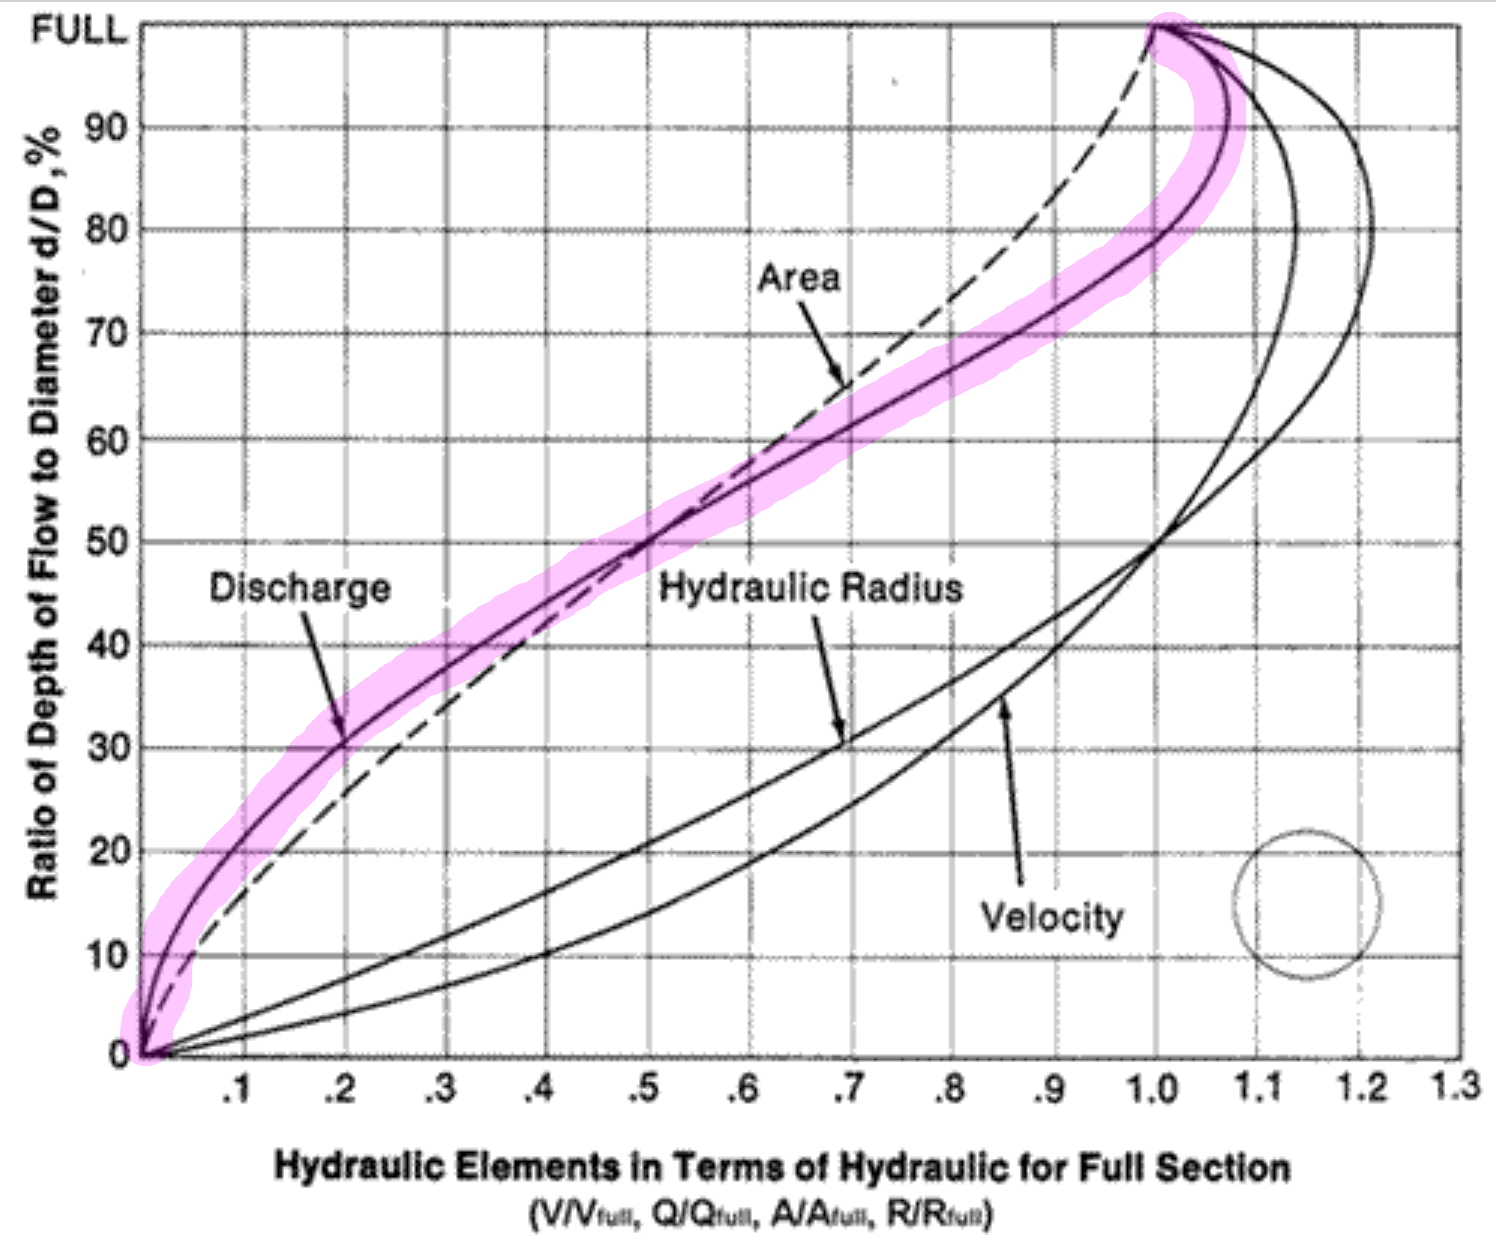
\includegraphics[height=5in]{hydraulic-elements-simple.jpg}
   \caption{Hydraulic elements chart}
   \label{fig:hydraulic-elements-simple} 
\end{figure}
\clearpage